%% LyX 2.1.4 created this file.  For more info, see http://www.lyx.org/.
%% Do not edit unless you really know what you are doing.
\documentclass[english]{article}
\usepackage{mathptmx}
\usepackage{helvet}
\usepackage{courier}
\usepackage[T1]{fontenc}
\usepackage[latin9]{inputenc}
\usepackage{geometry}
\geometry{verbose,tmargin=1in,bmargin=1in,lmargin=1in,rmargin=1in,headheight=0in,headsep=0in}
\pagestyle{empty}
\usepackage{babel}
\usepackage{graphicx}
\usepackage[unicode=true]
 {hyperref}

\makeatletter

%%%%%%%%%%%%%%%%%%%%%%%%%%%%%% LyX specific LaTeX commands.
%% Because html converters don't know tabularnewline
\providecommand{\tabularnewline}{\\}

%%%%%%%%%%%%%%%%%%%%%%%%%%%%%% Textclass specific LaTeX commands.
\newenvironment{lyxlist}[1]
{\begin{list}{}
{\settowidth{\labelwidth}{#1}
 \setlength{\leftmargin}{\labelwidth}
 \addtolength{\leftmargin}{\labelsep}
 \renewcommand{\makelabel}[1]{##1\hfil}}}
{\end{list}}

%%%%%%%%%%%%%%%%%%%%%%%%%%%%%% User specified LaTeX commands.
\date{}

\makeatother

\begin{document}
\begin{center}
\textbf{\large{}CSCE 221 Assignment 3 Cover Page}\\
\bigskip{}

\par\end{center}

First Name~~~~~~~~~~~~Chris~~~~~~~~~~Last Name
~~~~~~~Comeaux~~~~~~~~~UIN~~~~622006681~~~~~~~~~~\bigskip{}


User Name ~~~~~~~~cmc236~~~~~~~~~~~~~~~~~~~~~E-mail
address~~~~~~~cmc236@tamu.edu~~~~~~~~~~~~~~~~~~~~~~~\medskip{}


Please list all sources in the table below including web pages which
you used to solve or implement the current homework. If you fail to
cite sources you can get a lower number of points or even zero, read
more on Aggie Honor System Office website: \texttt{\href{http://aggiehonor.tamu.edu/}{http://aggiehonor.tamu.edu/}}\medskip{}
\medskip{}


\noindent \begin{flushleft}
\begin{tabular}{|c|c|c|}
\hline 
Type of sources  & ~~~~~~~~~~~~~~~~~~~~~~~ & ~~~~~~~~~~~~~~~~~~~~~~~~\tabularnewline
 &  & \tabularnewline
\hline 
People & Peer Teacher & Dr. Teresa Leyk\tabularnewline
 &  & \tabularnewline
\hline 
Web pages (provide URL)  & http://www.cplusplus.com/ & http://www.geeksforgeeks.org/618/\tabularnewline
 &  & \tabularnewline
\hline 
Web cont. & http://www.chegg.com/homework-help & http://stackoverflow.com/questions/19018294/c-to-check\tabularnewline
 & /definitions/binary-search-tree-3 & -if-user-input-is-a-number-not-a-character-or-a-symbol\tabularnewline
\hline 
Other Sources  &  & \tabularnewline
 &  & \tabularnewline
\hline 
\end{tabular}
\par\end{flushleft}

\medskip{}
\medskip{}


\noindent I certify that I have listed all the sources that I used
to develop the solutions/codes to the submitted work.

\noindent \emph{On my honor as an Aggie, I have neither given nor
received any unauthorized help on this academic work}.

\bigskip{}
\bigskip{}


\begin{tabular}{cccccc}
Your Name  & Chris &  & Comeaux & Date  & 3/19/2016\tabularnewline
\end{tabular}

\pagebreak{}


\section*{Assignment Objective}

The objective of this assignment is to create a Binary Search Tree
from scratch. In doing this students learn how to create a Binary
Search Tree, learn about recursive functions, and learn how to implement
recursive functions to do various tasks. The students then used the
Binary Search Tree class they created to create a simple program.
First the program read in a list of integers from a file. Then that
list was used to create a Binary Search Tree. As each node was being
entered into the tree, 3 things happened. First, the node was being
added to the tree, next the search cost for each node was being calculated,
and third, the size of the tree was being updated. Once the tree is
complete, the program outputs each node and its search cost. It then
uses preorder, postorder, and inorder traversals to output the tree
to either the screen or a file. Next the program calculates the average
search cost of the tree. Finally, the program asks the user to enter
a number to delete from the tree. It will update the tree, output
the final tree, and then terminate.


\section*{Purpose of the Assignment}

The purpose of the assignment was to grow student's knowledge of Binary
Trees. The students had to use their knowledge and understanding of
Binary Trees and recursive functions to write their own Binary Tree
class and write an application for it.


\section*{Instructions to Compile and Run your Program}

To compile the program, navigate to the PA4 directory using cd csce221/PA4.
Then just use the 'make' command. This will compile the program and
produce and executable file. To run the program, use the command ./Main.
The program will ask you which you would like to to open. Enter a
file name. Then the program will enter the data into the tree and
begin working on it. Then the program will ask you to enter a number
to remove from the tree. After the program has updated the tree, it
will then terminate.


\section*{Program Organization and Description of Classes }

I used two classes to create my Binary Search Tree. The first class,
BTreeNode, was used to create the individual tree node. It has a member
to hold key, a member to hold the search cost, and 3 members that
are pointers called left\_child, right\_child, and parent, which pointed
to the node's left child, right child, and parent respectfully. The
class also has member functions to help gain access to private members
and to check if the node is external or not. The next class, BSTree,
was used to create the actual tree structure. It has 2 members. One
member was the size of the tree and the other member was a pointer
to a BTreeNode called root, which was the root of the tree. BSTree
has multiple member functions. They help the user print, gain access
to its members, get the height of the tree, insert a node into the
tree, remove node from a tree, find the minimum node and remove it,
find the average search cost, and traverse the tree. Also, BSTree
is a friend class of BTreeNode, so it can access all of BTreeNode's
private members. Both classes, BTreeNode and BSTree, have their declarations
in BinarySearchTree.h. The implementation of BSTree is in BinarySeachTree.cpp,
however, since all of BTreeNodes helper function are defined in the
class, a separate .cpp file was not needed. 


\section*{Data Structure Description}

I created my Binary Search Tree using a Linked List type data structure.
Each node is linked to its two children and its parent through pointers.
The tree starts out as a single node called ``root.'' When a node
is inserted into a tree, it is only simply linked by the left\_child
or right\_child pointers and the parent pointer. In other words, the
data can be in any place in memory (i.e. does not have to be in a
sequence of bites). As described in the previous section, the BTreeNode
class represents the individual nodes of the tree, and the BSTree
represents the nodes linked together to form a tree.


\section*{Calculations}
\begin{itemize}
\item \textbf{Individual Search Cost}: The individual search cost of each
node was calculated in the insert\_node function. Insert\_node is
implemented by recursion. If the function does not find the right
place to enter the node it calls itself with either its left or right
child. Every time it is called the it keeps track of the previous
nodes search cost. This allows the function to simple add one to the
parents search cost when initializing the new node and adding it to
the tree.
\item \textbf{Average Search Cost: }The average search cost has two parts,
the size and the total search cost of the tree. To calculate the size,
I added one to the tree's member 'size' every time the a node was
inserted and subtracted one from 'size' every time a node was removed.
The total search cost is calculated in the postOrder function. Every
time it outputs a node, it also accesses the nodes search cost and
adds it to the tree's member 'TotalSC', which holds the total search
cost of the tree. Once these two values have been calculated, the
average search cost is calculated in the function aveSC. It simple
returns the 'TotalSC' divided by 'size'.
\item \textbf{Updated Search Cost:} This does not apply to my class because
in my implementation of my binary tree, when a node is removed, the
search costs of the nodes are not affected. With a perfect or a random
tree, the remove function simply switches the keys of the deleted
node with the left child's key (if it is an external node) or switches
the key with the least node in the right sub-tree the deletes that
node. The search costs of the nodes are not affected. For a linear
tree, the keys of the nodes below the deleted nodes are simple shifted
up one and the last node is deleted. 
\end{itemize}

\section*{Time Complexity}
\begin{itemize}
\item \textbf{Individual Search Cost}: The time complexity of calculating
the individual search cost would be O(log(n)) where n is the number
of nodes in the tree at that point. This is because, on average, about
half of the nodes have to be visited for a node to be inserted into
the tree and since the search cost is calculated during insertion,
it will have the same Big-O notation as the insertion function.
\item \textbf{Updated Search Cost: }The time complexity of updating the
search cost would be same as deleting a node from the tree. The Big-O
notation would be O(log(n)) where n is the number of nodes in the
tree at that point. This is because, on average, about half of the
nodes have to be visited for a node to be deleted from the tree.
\item \textbf{Summing Up Search Cost: }The time complexity of summing up
the search cost of the tree is O(n) where n is the number of nodes
in the tree at that point. This is because every node must be visited
inorder to sum up all the search costs.
\end{itemize}

\section*{Search Costs}

If we let n be the individual search cost of each node of a binary
tree, then the best and average case for a binary tree would be O(log(n)).
These cases are would result from a perfect and random binary tree.
The worst case for a binary tree would be O(n), which comes with a
linear tree. For the perfect tree and random tree (best and average
cases), the height is log(n), on each level there are 2\textasciicircum{}k
nodes, and the total search time is (log1+1) + 2(log2+1) + 2\textasciicircum{}2(log3+1)
+ 2\textasciicircum{}3(log4) +...+ 2\textasciicircum{}(log(n+1)) -
1(log(n)+1) = (n+1)log(n+1) - n. This means that the average time
is O(log(n)). For the linear tree (worst case), the height is n-1
and the total search cost is n(n+1)/2. Dividing these you would get
(n+2)/2 which is O(n). 


\section*{Graphs and Tables}

After analyzing the tables and graphs we see that the theoretical
results in part 4 match the results shown here. Analyzing both the
Perfect and Random trees (Best and Average case respectfully) we see
that they are both O(log(n)) which is what we found in part 4. Analyzing
the Linear tree (worst case) we see that the average case for the
Linear tree is 2n which is O(n) which is also what we found in part
4. 
\begin{lyxlist}{00.00.0000}
\item [{%
\begin{tabular}{|c||c|c|c|}
\hline 
Nodes  & Perfect  & Random  & Linear \tabularnewline
\hline 
\hline 
1  & 1  & 1  & 1 \tabularnewline
\hline 
3  & 1.66667 & 1.66667 & 2 \tabularnewline
\hline 
7  & 2.42857  & 2.71429  & 4 \tabularnewline
\hline 
15  & 3.26667  & 3.73333  & 8\tabularnewline
\hline 
31  & 4.16129  & 6.3871  & 16\tabularnewline
\hline 
63  & 5.09524  & 7.66667  & 32\tabularnewline
\hline 
127  & 6.05512  & 7.59055  & 64\tabularnewline
\hline 
255  & 7.03137  & 9.06667  & 128\tabularnewline
\hline 
511  & 8.01761  & 10.3033  & 256\tabularnewline
\hline 
1023 & 9.00978  & 12.2463  & 512\tabularnewline
\hline 
2047 & 10.0054  & 13.3972  & 1024\tabularnewline
\hline 
4095 & 11.0029  & 14.0237  & 2048\tabularnewline
\hline 
\end{tabular}}]~
\end{lyxlist}
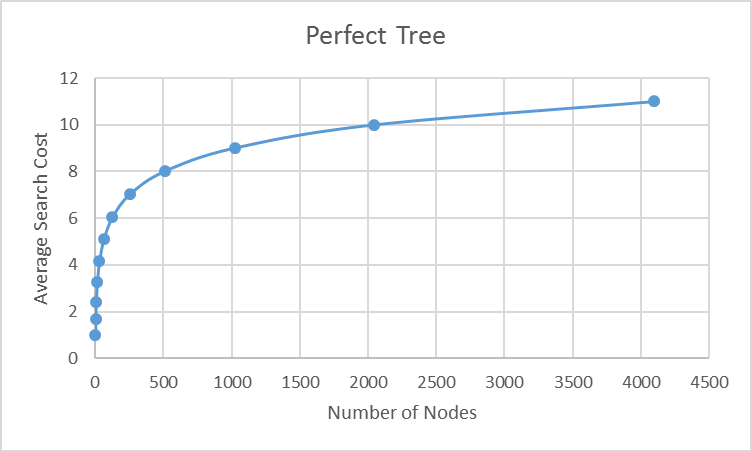
\includegraphics{Perfect}\newline

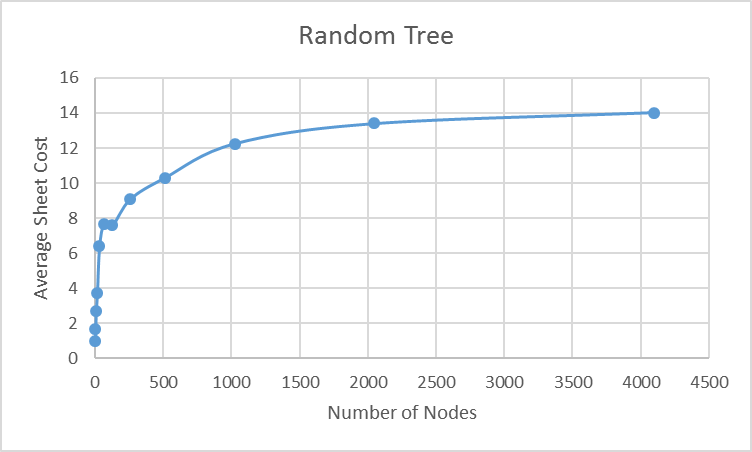
\includegraphics{Random}\newline

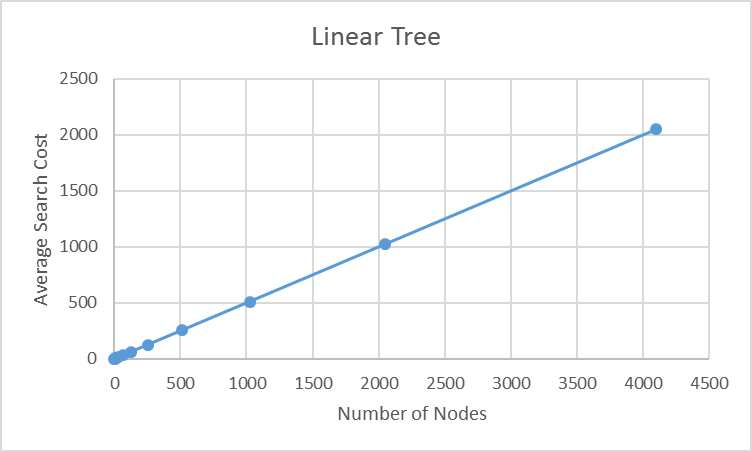
\includegraphics{Linear}
\end{document}
